\section{Noise Modeling}
\noindent
In our quality control analysis, we were interesting to remove the noise
from the BOLD images. 
We first detect the voxels which are inside of the brain. We did not know
if the threshold would be the same accross all subjects and runs. After 
plotting a few histograms of the mean value of the voxels accross time 
for different subject and runs, we settle for a common threshold value of
300.
\begin{figure}[H]
    \centering
        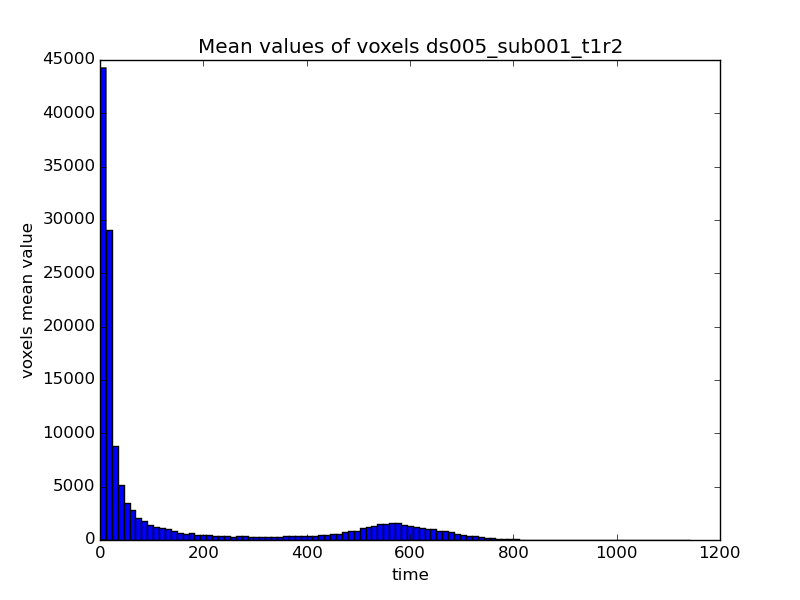
\includegraphics[scale=0.4]{../plots/ds005_sub001_t1r2_hist.png}
            \caption{Histogram of mean voxels accross time - subject1 - run1 }
\end{figure}

Applying the mask on the image data allow us to select only the voxels that
are in the brain. 
We then model our signal with some additional drift terms to account for
the subject head motion in the scanner. We deceide to add a linear and a 
quadratic drift terms as regressors. The following brain images justify
our design decision.

\begin{figure}[H]
    \centering
        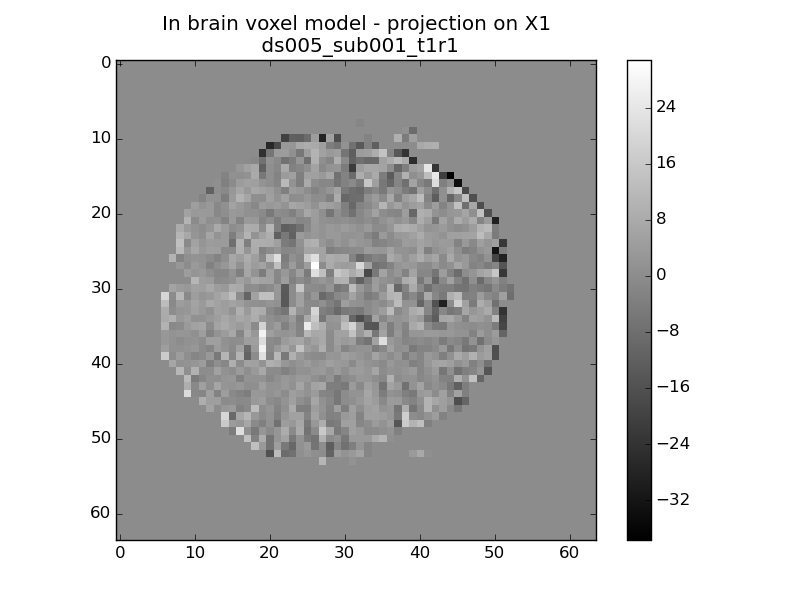
\includegraphics[scale=0.5]{../plots/ds005_sub001_t1r1_noise_modelX1.png}
             \caption{Projection of the brain image on the linear drift related regressor - subject1 - run1}
\end{figure}

The above image illustrates the effect of the linear drift regressor on the BOLD image.
Lighter pixels indicates a higher position of the zone compare
to darker zones. We can clearly see the edges of the top right of the brain to be
dark (black) and the edges on the bottom left of the brain to be light (white). 
This suggests a clear linear movement of the head in the direction of the axis. 

\begin{figure}[H]
    \centering
        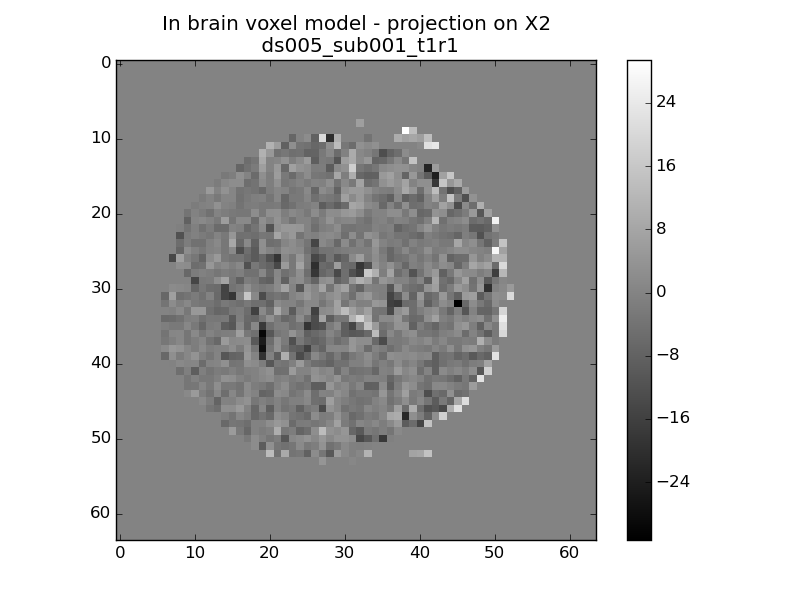
\includegraphics[scale=0.5]{../plots/ds005_sub001_t1r1_noise_modelX2.png}
            \caption{Projection of the brain image on the linear drift related regressor - subject1 - run1}
\end{figure}

The aboce image clearly illustrates a strong influence on the quadratic regressor in
the design matrix. We can clearly distinguish light and dark areas on the above images.

Our design matrix includes the above drift regressors in order to get a more accurate
estimation of the task which effects will not be confounded with the movement of the
brain.

